\documentclass[12pt]{article}
\usepackage[top=1in, bottom=1in, left=1in, right=1in]{geometry}

\usepackage{setspace}
\onehalfspacing

\usepackage{amssymb}
%% The amsthm package provides extended theorem environments
\usepackage{amsthm}
\usepackage{epsfig}
\usepackage{times}
\renewcommand{\ttdefault}{cmtt}
\usepackage{amsmath}
\usepackage{graphicx} % for graphics files
\usepackage{tabu}

% Draw figures yourself
\usepackage{tikz} 

% writing elements
\usepackage{mhchem}

\usepackage{paralist}

% The float package HAS to load before hyperref
\usepackage{float} % for psuedocode formatting
\usepackage{xspace}

% from Denovo Methods Manual
\usepackage{mathrsfs}
\usepackage[mathcal]{euscript}
\usepackage{color}
\usepackage{array}

\usepackage[pdftex]{hyperref}
\usepackage[parfill]{parskip}

% math syntax
\newcommand{\nth}{n\ensuremath{^{\text{th}}} }
\newcommand{\ve}[1]{\ensuremath{\mathbf{#1}}}
\newcommand{\Macro}{\ensuremath{\Sigma}}
\newcommand{\rvec}{\ensuremath{\vec{r}}}
\newcommand{\omvec}{\ensuremath{\hat{\Omega}}}
\newcommand{\vOmega}{\ensuremath{\hat{\Omega}}}
%---------------------------------------------------------------------------
%---------------------------------------------------------------------------
\begin{document}
\begin{center}
{\bf NE 255, Fa16 \\
Equation Discretization\\
September 22, 2016}
\end{center}

\setlength{\unitlength}{1in}
\begin{picture}(6,.1) 
\put(0,0) {\line(1,0){6.25}}         
\end{picture}

Start from the general time-dependent NTE without delayed neutrons, with 7 independent variables. We need to discretize each variable.	
%
\begin{align}
&\frac{1}{v}\frac{\partial \psi}{\partial t}(\rvec,E,\omvec,t) + 
\omvec\cdot  \nabla \psi(\rvec,E,\omvec,t)+
\Sigma_t(\rvec,E)\psi(\rvec,E,\omvec,t)
\\& \quad\quad\quad\quad =
\int_0^{\infty}\int_{4\pi}\Sigma_s(\rvec, E'\rightarrow E,\omvec'\rightarrow\omvec)
\psi(\rvec,E',\omvec',t)d\omvec'dE'\nonumber
\\&\quad\quad\quad\quad\quad\quad +\frac{\chi_p(E)}{4\pi}\int_0^{\infty}\int_{4\pi}\nu(E')\Sigma_f(\rvec,E')
\psi(\rvec,E',\omvec',t)d\omvec'dE'\nonumber
\\&\quad\quad\quad\quad\quad\quad\quad\quad+S(\rvec, E, \omvec,t)\nonumber.
\end{align}

\subsection*{Time}
Discretize the time interval $[0, T]$ into $N$ timesteps:
%
\begin{figure}[h!]
    \begin{center}
    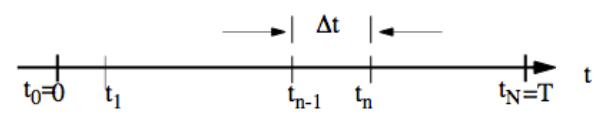
\includegraphics[keepaspectratio, width = 3.5 in]{time}
    \end{center}
\end{figure}
%
Integrate the equation from $t=t_{n-1}$ to $t = t_n$, where we will use the following definitions:
\begin{align*}
\psi(\vec{r}, E ,\vOmega, t_n) &= \psi_n(\vec{r}, E ,\vOmega)\\
\Delta t &= t_{n} - t_{n-1}\\
\bar{\psi}(\vec{r}, E ,\vOmega) &= \frac{1}{\Delta t} \int_{t_{n-1}}^{t_n} dt\: \psi(\vec{r}, E ,\vOmega, t)
\end{align*}
(Note that this integration is functionally ignoring what actually happens in the integration by giving us a time-averaged angular flux; we don't care about more details than that).

To update the equation we simply convert each term to this time-averaged angular flux \textit{except} the term containing a time derivative. We need to handle that specially by using \textit{First Order Backward Difference}: 
\[
\frac{1}{v} \int_{t_{n-1}}^{t_n} dt\:\frac{\partial \psi}{\partial t}(\rvec,E,\omvec,t) = \frac{1}{v}\frac{\psi_n(\vec{r}, E ,\vOmega) - \psi_{n-1}(\vec{r}, E ,\vOmega)}{\Delta t}
\]
Combining all of that we get the following:
\begin{align*}
\frac{1}{v}&\frac{\psi_n(\vec{r}, E ,\vOmega) - \psi_{n-1}(\vec{r}, E ,\vOmega)}{\Delta t} 
+ \omvec\cdot  \nabla  \bar{\psi}(\vec{r}, E ,\vOmega) 
+ \Sigma_t(\rvec,E)\bar{\psi}(\vec{r}, E ,\vOmega) 
= \\& \int_0^{\infty}dE'\int_{4\pi}d\omvec'\: \Sigma_s(\rvec, E'\rightarrow E,\omvec'\rightarrow\omvec) \bar{\psi}(\vec{r}, E' ,\vOmega')
\\&+ \frac{\chi_p(E)}{4\pi}\int_0^{\infty}dE'\:\nu(E')\Sigma_f(\rvec,E')\int_{4\pi}d\omvec'\:
\bar{\psi}(\vec{r}, E' ,\vOmega')
+\bar{S}(\rvec, E, \omvec)
\end{align*}
Note(!): we now have two unknowns ($\psi_n$ and $\bar{\psi}$). We need to relate them; we choose a linear combination with a weighting parameter, $\beta$:
\[
\bar{\psi} = \beta \psi_n + (1 - \beta)\psi_{n-1}
\]
We substitute this in to get
\begin{align*}
\omvec\cdot  \nabla  \bar{\psi}(\vec{r}, E ,\vOmega) 
&+ \bigl(\Sigma_t + \frac{1}{v \beta \Delta t}\bigr)\bar{\psi}(\vec{r}, E ,\vOmega) 
=  \frac{1}{v \beta \Delta t} \psi_{n-1}(\vec{r}, E ,\vOmega) \\
&+ \int_0^{\infty}dE'\int_{4\pi}d\omvec'\: \Sigma_s(\rvec, E'\rightarrow E,\omvec'\rightarrow\omvec) \bar{\psi}(\vec{r}, E' ,\vOmega')
\\&+ \frac{\chi_p(E)}{4\pi}\int_0^{\infty}dE'\:\nu(E')\Sigma_f(\rvec,E')\int_{4\pi}d\omvec'\:
\bar{\psi}(\vec{r}, E' ,\vOmega')
+\bar{S}(\rvec, E, \omvec)
\end{align*}


%---------------------------------------------------------------------------
\subsubsection*{Aside about Finite Difference}
Finite difference is a common way to numerically approximate derivatives.  \textbf{Example} Given $f$ is $ C^2 \in [a,b]$ and $x_0 \in [a,b]$, find an approximation to $f'(x_0)$ and or $f''(x_0)$, etc.

We're going to come at this from \textbf{Taylor's theorem}, which gives an approximation of a k-times differentiable function around a given point by a k-th order Taylor polynomial.
\[
f(x) = \sum_{0}^{k} \frac{f^{(n)}(x_0)}{n!}(x - x_0)^n
\]
% https://en.wikipedia.org/wiki/Taylor%27s_theorem
To approximate any type of derivative to a specified order of accuracy, we Taylor expand several points in our collection. Then, we choose how many points to combine and in what ways. 
\begin{align*}
f(x_0) &= f(x_0)\\
%
f(x_0 \pm h) &= f(x_0) \pm hf'(x_0) + h^2\frac{f''(x_0)}{2} \pm h^3\frac{f'''(x_0)}{6} + f^{(4)}(c_1)\frac{h^4}{24} \\
%
f(x_0 \pm 2h) &= f(x_0) \pm 2h f'(x_0) + 2 h^2 f''(x_0) \pm \frac{4}{3} h^3 f'''(x_0) + \frac{2}{3}h^4 f^{(4)}(c_2)
\end{align*}
We combine the expanded expressions, rearrange to group terms, and solve for what we want:

For \underline{$O(h)$ Backwards Difference}: combine the point and the next point backward:
\begin{align*}
f(x_0) &= f(x_0)\\
f(x_0 - h) &= f(x_0) - hf'(x_0) + h^2\frac{f''(c)}{2}\\
a f(x_0) &+ b f(x_0 - h) = f'(x_0) \\
a f(x_0) &+ b \bigl(f(x_0) - hf'(x_0) + h^2\frac{f''(c)}{2} \bigr) = f'(x_0) \\
(a+b)f(x_0) &-bh f'(x_0) + b h^2\frac{f''(c)}{2} = f'(x_0)
\end{align*}
%
Now, we solve for the coefficients to get what we want
\begin{align*}
a+b = 0 &\quad -bh = 1 \\
b &= -\frac{1}{h} \quad a = \frac{1}{h}
\end{align*}
%
We now sub in $a$ and $b$. This gives the first order ($O(h)$) Backwards Difference approximation, which is what we used for the time derivative.
\begin{align*}
\text{error }&= -\frac{1}{h}h^2\frac{f''(c)}{2}\\
f'(x_0) &= \frac{f(x_0) - f(x_0 - h)}{h} + \frac{1}{2}hf''(\mu)
\end{align*}


%---------------------------------------------------------------------------
%---------------------------------------------------------------------------
\subsection*{Energy Discretization}


\end{document}